\subsection{Applying Wick's theorem for the interaction term}
Let's apply Wick's theorem to calculate the next term in the series of our quantity \[ \bra{0} \mathcal{T} \phi(x) \phi(y) \exp \left(  -i  \int dt H_I(t) \right) \ket{0} \] . Let's resume our discussion in the case of $\phi^4$ theory, where our interaction Hamiltonian is $\int d^3 z \phi^4(z) $. Recall, our first term in the series expansion is just \[ \bra{0} \phi(x) \phi(y) \ket{0} = \Delta_F(x -y)  \] and our expression in the series expansion is \[ \bra{0} -i\frac{ \lambda} { 4!}   \mathcal{T} \phi(x) \phi(y)  \int dt \int d^3 z \phi^4 (z) \ket{0} \]       
We can write this a little more concisely by combining writing $\int dt \int d^3z = \int d^4 z$, so we're aware that it's an integral over four space time dimensions. To make it clearer to understand the nature of the contractions in this expression, we do something a bit weird and write out the terms in the $\phi^4$ term as $\phi(z)\phi(z)\phi(z) \phi(z)$. 
We want to cookup a simplified expression for the term \[  - i \frac{ \lambda} {4!} \bra{0}\mathcal{T} \phi(x) \phi(y) \int d^4 z \phi(z) \phi(z) \phi(z) \phi(z) \ket{0} \] Since we have a time ordering operator there, the only non zero terms which surivive once we expand this thing into a sum are the terms where every scalar $\phi$ in contracted with another. The important thing to remember is that this includes the $\phi(z) $ terms incorporated into the integral. There are several contraction we could do here, but the most obvious one to start with is to first contract $\phi(x)$ and $\phi(y)$ together, and then pair up the terms in the integral as follows \[ 
- \frac{ i \lambda} { 4!} \contraction{}{\phi(x) }{} { \phi(y) } \phi(x) \phi(y) \int d^4 z \contraction{}{\phi(z)}{} { \phi(z) } \phi(z) \phi(z) \contraction{}{\phi(z) }{}{\phi(z) } \phi(z) \phi(z) \] but this corresponds to, replacing the contractions with Feynman propagators, \[ - \frac{i \lambda} { 4!} \Delta_F( x - y ) \int d^4 \Delta_F(z - z) \Delta_F(z - z) \] 
Alternatively, we could have contracted the $\phi(z)$ terms differently in the integrand, and instead could have contracted the terms like so: 
\[ - i \frac{ \lambda} { 4!} \contraction{}{\phi(x) }{ } {\phi(y) } \phi(x) \phi(y)  \int d^4 z \contraction{} {\phi(z)}{\phi(z)}{ \phi(z) }  \contraction[2ex]{\phi(z)}{\phi(z)}{\phi(z)}{\phi(z) } \phi(z) \phi(z) \phi(z) \phi(z) \] 
This term here still corresponds to the integral  \[ - \frac{i \lambda} { 4!} \Delta_F( x - y ) \int d^4 z \Delta_F(z - z) \Delta_F(z - z) \]
We count that there are in total 3 different sets of contractions which yield this integral. So the contribution that we have from contractions of this type is  \[ - \frac{3 i \lambda} { 4!} \Delta_F( x - y ) \int d^4 z  \Delta_F(z - z) \Delta_F(z - z) \]   
We represent this type of contraction diagramatically like before in the following diagram.

\begin{figure}[!h] 
\centering
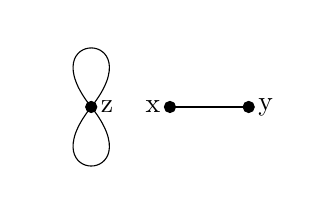
\begin{tikzpicture}
\filldraw[black] (0, 0) circle (2pt) node[anchor=west] {z} ; 
\draw (0, 0) .. controls (0.8, 1) and (-0.8, 1) .. (0, 0);
\draw (0, 0) .. controls (0.8, -1) and (-0.8, -1) .. (0, 0); 

\filldraw[black] (1, 0) circle (2pt) node[anchor=east] {x} ; 
\filldraw[black] (2, 0) circle (2pt) node[anchor=west] {y} ; 
\draw (1, 0) -- (2, 0) ; 
\end{tikzpicture}  
\end{figure} 

We also have another type of contraction that we can include. We contract $\phi(x)$ with one of the $\phi(z)$, and contract $\phi(y) $ with another one. This gives us $12$ choices for our contraction. One of these may look like \[  - \frac{i \lambda}{ 4!} \contraction[2ex]{}{\phi(x) } {\phi(y) \int d^4 z \, }{ \phi(z) } \contraction[3ex]{ \phi(x) } { \phi(y) } { \int d^4 z \, phi(z ) }{\phi(z)} \phi(x) \phi(y ) \int d^4 z \, \phi(z) \phi(z) \contraction{}{\phi(z)} {} {\phi(z)} \phi(z) \phi(z)  \] we count 12 of these, and represent this diagramatically in the figure adjacent.  
\begin{figure}[!h] 
\centering
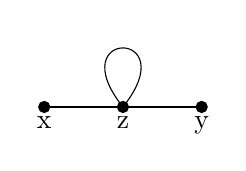
\begin{tikzpicture}
\filldraw[black] (0, 0) circle (2pt) node[anchor=north] {x}; 
\filldraw[black] (1, 0) circle (2pt) node[anchor=north] {z}; 
\filldraw[black] (2, 0) circle (2pt) node[anchor=north] {y}; 

\draw (0, 0) -- (1, 0); 
\draw (1, 0) -- (2, 0); 

\draw (1, 0) .. controls (0.2, 1) and (1.8, 1) .. (1, 0) ; 
\end{tikzpicture}
\end{figure} 
Our total first order contribution is therefore \[ - \frac{ 3i\lambda }{ 4!} D_F(x - y )  \int d^4 z \, D_F(z - z)  D_F(z - z) - \frac{12 i \lambda}{ 4! } \int d^4 z \, D_F( x - z) D_F( y - z) D_F( z - z ) \] which exhausts all of the possible ways to contract terms in our sum above. 

\subsubsection{Symmetry factors} 
We now present a convinient way to find the coefficent of our contribution which a diagram contributes. This is called the symmetry factor of the diagram. It is as follows. Given a particular diagram, 
\begin{enumerate} 
\item Ascribe a symmetry factor of 2 for edges which loop to the same node. 
\item Ascribe a symmetry factor of $n$ for edges which can be interchanged
\item Ascribe a symmetry factor of 2 for vertices which are equivalent. 
\end{enumerate}
As an example, consider the diagram below. 

\pagebreak
